\documentclass[11pt]{article}

\usepackage[margin=1in]{geometry}
\usepackage{graphicx}
\usepackage{array}
\usepackage{longtable}
\usepackage{hyperref}
\usepackage{booktabs}
\usepackage{xcolor}
\usepackage{tikz}
\usepackage{float}
\usepackage{enumitem}
\usepackage{fancyhdr}
\usepackage{titlesec}
\usepackage{tcolorbox}
\usepackage{tabularx}
\usepackage{multirow}
\usepackage{caption}
\usepackage{subcaption}
\usepackage{listings}
\usepackage{makecell}
\usepackage{amssymb}
\usepackage{pifont}

\usetikzlibrary{shapes.geometric, arrows.meta, positioning, fit, backgrounds, calc, decorations.pathreplacing, shapes.multipart, matrix, shadows, trees, patterns}

% Color definitions
\definecolor{variationcolor}{RGB}{70,130,180}
\definecolor{variantcolor}{RGB}{60,179,113}
\definecolor{bindingcolor}{RGB}{255,165,0}
\definecolor{constraintcolor}{RGB}{186,85,211}
\definecolor{flowcolor}{RGB}{100,100,100}
\definecolor{sectionblue}{RGB}{31,78,121}
\definecolor{lightgray}{RGB}{245,245,245}
\definecolor{warningred}{RGB}{220,53,69}
\definecolor{successgreen}{RGB}{40,167,69}
\definecolor{infoblue}{RGB}{23,162,184}
\definecolor{mandatorycolor}{RGB}{0,123,255}
\definecolor{optionalcolor}{RGB}{108,117,125}
\definecolor{alternativecolor}{RGB}{255,193,7}
\definecolor{orcolor}{RGB}{220,53,69}
\definecolor{compiletime}{RGB}{144,238,144}
\definecolor{deploytime}{RGB}{255,218,185}
\definecolor{runtime}{RGB}{173,216,230}

% Hyperref setup
\hypersetup{
    colorlinks=true,
    linkcolor=sectionblue,
    urlcolor=sectionblue,
    citecolor=sectionblue
}

% Header and footer
\pagestyle{fancy}
\fancyhf{}
\fancyhead[L]{\leftmark}
\fancyhead[R]{Variability Guide Documentation}
\fancyfoot[C]{\thepage}
\renewcommand{\headrulewidth}{0.4pt}
\renewcommand{\footrulewidth}{0.4pt}

% Section formatting
\titleformat{\section}
  {\normalfont\Large\bfseries\color{sectionblue}}{\thesection}{1em}{}
\titleformat{\subsection}
  {\normalfont\large\bfseries\color{sectionblue!80}}{\thesubsection}{1em}{}
\titleformat{\subsubsection}
  {\normalfont\normalsize\bfseries\color{sectionblue!60}}{\thesubsubsection}{1em}{}

% Custom box environments
\newtcolorbox{keypoint}{
    colback=blue!5,
    colframe=sectionblue,
    title=Key Point,
    fonttitle=\bfseries
}

\newtcolorbox{warning}{
    colback=red!5,
    colframe=warningred,
    title=Warning,
    fonttitle=\bfseries
}

\newtcolorbox{bestpractice}{
    colback=green!5,
    colframe=successgreen,
    title=Best Practice,
    fonttitle=\bfseries
}

\newtcolorbox{example}{
    colback=lightgray,
    colframe=flowcolor,
    title=Example,
    fonttitle=\bfseries
}

\newtcolorbox{definition}{
    colback=infoblue!10,
    colframe=infoblue,
    title=Definition,
    fonttitle=\bfseries
}

\newtcolorbox{template}{
    colback=white,
    colframe=flowcolor,
    title=Template,
    fonttitle=\bfseries
}

\newtcolorbox{variationbox}[1][]{
    colback=variationcolor!10,
    colframe=variationcolor,
    title=#1,
    fonttitle=\bfseries,
    breakable
}

\newtcolorbox{configbox}[1][]{
    colback=variantcolor!10,
    colframe=variantcolor,
    title=#1,
    fonttitle=\bfseries
}

% Code listing style
\lstset{
    basicstyle=\ttfamily\small,
    breaklines=true,
    frame=single,
    backgroundcolor=\color{lightgray},
    keywordstyle=\color{sectionblue},
    commentstyle=\color{successgreen},
    stringstyle=\color{bindingcolor},
    showstringspaces=false
}

% Custom column types
\newcolumntype{L}[1]{>{\raggedright\arraybackslash}p{#1}}
\newcolumntype{C}[1]{>{\centering\arraybackslash}p{#1}}
\newcolumntype{R}[1]{>{\raggedleft\arraybackslash}p{#1}}

% Feature model symbols
\newcommand{\mandatory}{\textcolor{mandatorycolor}{\ding{108}}}
\newcommand{\optional}{\textcolor{optionalcolor}{\ding{109}}}
\newcommand{\alternative}{\textcolor{alternativecolor}{\ding{115}}}
\newcommand{\orfeature}{\textcolor{orcolor}{\ding{116}}}

\title{%
    \vspace{-1cm}
    \textbf{\Huge Software Architecture Documentation}\\[12pt]
    \Large Variability Guide\\[8pt]
    \large A Comprehensive Guide to Documenting Architectural\\
    Variability, Configuration, and Product Line Flexibility
}
\author{%
    \textit{Architecture Documentation Series}\\[4pt]
    \small Based on Software Product Line Engineering, Feature Modeling, and Industry Best Practices
}
\date{\today}

\begin{document}

\maketitle
\thispagestyle{empty}

\vspace{0.8cm}

\begin{abstract}
\noindent
The Variability Guide documents how an architecture accommodates variation---the deliberate flexibility built into a system to support different configurations, product variants, deployment environments, and customer customizations. Effective variability management is essential for software product lines, configurable systems, and platforms that must serve diverse needs without fragmenting into unmaintainable branches. This comprehensive guide establishes principles and practices for documenting variation points, binding times, allowed variants, configuration mechanisms, and constraints. The document covers feature modeling, variation point taxonomy, binding time analysis, configuration management strategies, constraint specification, and governance processes for maintaining variability throughout the system lifecycle. Whether building a product line, a configurable enterprise system, or a multi-tenant platform, this guide provides the foundation for systematic variability documentation.
\end{abstract}

\vfill

\begin{center}
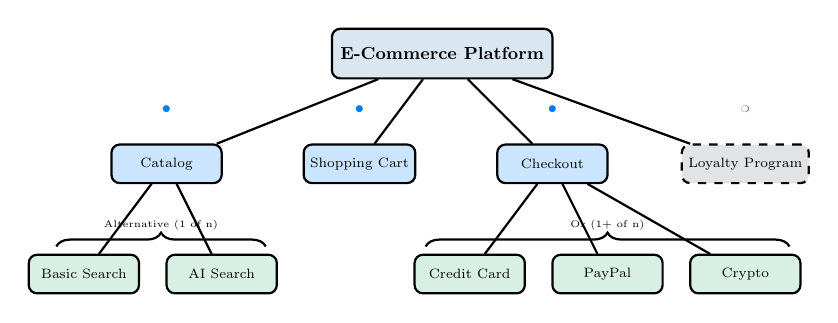
\begin{tikzpicture}[
    scale=0.7,
    transform shape,
    feature/.style={draw, thick, fill=variationcolor!20, minimum width=2.5cm, minimum height=0.9cm, rounded corners=3pt, font=\small},
    variant/.style={draw, thick, fill=variantcolor!20, minimum width=2cm, minimum height=0.7cm, rounded corners=3pt, font=\scriptsize},
    mandatory/.style={draw, thick, fill=mandatorycolor!20, minimum width=2cm, minimum height=0.7cm, rounded corners=3pt, font=\scriptsize},
    optional/.style={draw, thick, fill=optionalcolor!20, minimum width=2cm, minimum height=0.7cm, rounded corners=3pt, font=\scriptsize, dashed},
    arrow/.style={-, thick}
]
    % Root
    \node[feature, minimum width=4cm] (root) at (0,4) {\textbf{E-Commerce Platform}};
    
    % Level 1 - Mandatory features
    \node[mandatory] (catalog) at (-5,2) {Catalog};
    \node[mandatory] (cart) at (-1.5,2) {Shopping Cart};
    \node[mandatory] (checkout) at (2,2) {Checkout};
    \node[optional] (loyalty) at (5.5,2) {Loyalty Program};
    
    % Level 2 - Variants
    \node[variant] (search) at (-6.5,0) {Basic Search};
    \node[variant] (advsearch) at (-4,0) {AI Search};
    
    \node[variant] (cc) at (0.5,0) {Credit Card};
    \node[variant] (paypal) at (3,0) {PayPal};
    \node[variant] (crypto) at (5.5,0) {Crypto};
    
    % Connections
    \draw[arrow] (root) -- (catalog);
    \draw[arrow] (root) -- (cart);
    \draw[arrow] (root) -- (checkout);
    \draw[arrow] (root) -- (loyalty);
    
    \draw[arrow] (catalog) -- (search);
    \draw[arrow] (catalog) -- (advsearch);
    
    \draw[arrow] (checkout) -- (cc);
    \draw[arrow] (checkout) -- (paypal);
    \draw[arrow] (checkout) -- (crypto);
    
    % Cardinality indicators
    \node[font=\tiny, fill=white] at (-5,3) {\mandatory};
    \node[font=\tiny, fill=white] at (-1.5,3) {\mandatory};
    \node[font=\tiny, fill=white] at (2,3) {\mandatory};
    \node[font=\tiny, fill=white] at (5.5,3) {\optional};
    
    % Group indicators
    \draw[thick, decorate, decoration={brace, amplitude=5pt}] (-7,0.5) -- (-3.2,0.5) node[midway, above=5pt, font=\tiny] {Alternative (1 of n)};
    \draw[thick, decorate, decoration={brace, amplitude=5pt}] (-0.3,0.5) -- (6.3,0.5) node[midway, above=5pt, font=\tiny] {Or (1+ of n)};
\end{tikzpicture}
\end{center}

\newpage
\tableofcontents
\newpage

%==============================================================================
\section{Introduction to Variability}
%==============================================================================

\subsection{Definition and Purpose}

Variability in software architecture refers to the ability of a system or architecture to be efficiently extended, changed, customized, or configured for use in a particular context. The Variability Guide documents how this flexibility is designed into the architecture and how it should be exercised.

\begin{definition}
\textbf{Architectural Variability} is the deliberate design of flexibility into a software architecture, enabling a single architecture to support multiple products, configurations, deployments, or customizations through well-defined variation points that can be bound at various times in the software lifecycle.
\end{definition}

The Variability Guide serves several critical purposes. First, it enables \textbf{product line engineering} by documenting how a single architecture supports multiple products. Second, it supports \textbf{configuration management} by specifying what can be configured and how. Third, it facilitates \textbf{deployment flexibility} by explaining environment-specific variations. Fourth, it enables \textbf{customization} by defining how customer-specific adaptations are achieved. Fifth, it supports \textbf{evolution} by identifying extension points for future capabilities.

\subsection{The Business Case for Variability}

Well-managed variability provides significant business value through several mechanisms. It enables \textbf{mass customization} by allowing products to be tailored to customer needs without custom development. It accelerates \textbf{time-to-market} by enabling new product variants to be derived from existing assets. It reduces \textbf{maintenance costs} by sharing core components across product variants. It provides \textbf{market segmentation} by supporting different feature sets for different market segments. Finally, it ensures \textbf{future-proofing} by making the system adaptable to changing requirements.

\begin{figure}[H]
\centering
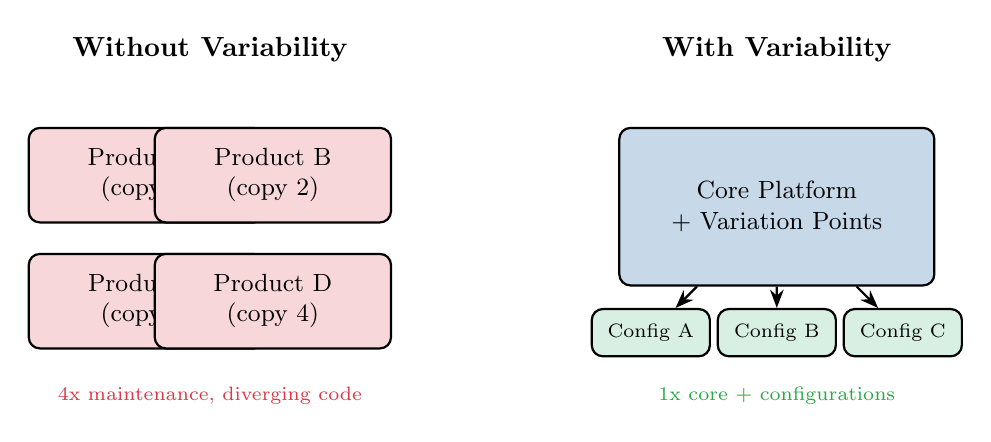
\begin{tikzpicture}[
    scale=0.8,
    box/.style={draw, thick, rounded corners, minimum width=3cm, minimum height=1.2cm, align=center, font=\small}
]
    % Without variability
    \node[font=\bfseries] at (-5,3) {Without Variability};
    \node[box, fill=warningred!20] (p1) at (-6,1) {Product A\\(copy 1)};
    \node[box, fill=warningred!20] (p2) at (-4,1) {Product B\\(copy 2)};
    \node[box, fill=warningred!20] (p3) at (-6,-1) {Product C\\(copy 3)};
    \node[box, fill=warningred!20] (p4) at (-4,-1) {Product D\\(copy 4)};
    
    % With variability
    \node[font=\bfseries] at (4,3) {With Variability};
    \node[box, fill=variationcolor!30, minimum width=4cm, minimum height=2cm] (core) at (4,0.5) {Core Platform\\+ Variation Points};
    \node[box, fill=variantcolor!20, minimum width=1.5cm, minimum height=0.6cm, font=\scriptsize] (v1) at (2,-1.5) {Config A};
    \node[box, fill=variantcolor!20, minimum width=1.5cm, minimum height=0.6cm, font=\scriptsize] (v2) at (4,-1.5) {Config B};
    \node[box, fill=variantcolor!20, minimum width=1.5cm, minimum height=0.6cm, font=\scriptsize] (v3) at (6,-1.5) {Config C};
    
    \draw[-{Stealth}, thick] (core) -- (v1);
    \draw[-{Stealth}, thick] (core) -- (v2);
    \draw[-{Stealth}, thick] (core) -- (v3);
    
    % Annotations
    \node[font=\scriptsize, text=warningred] at (-5,-2.5) {4x maintenance, diverging code};
    \node[font=\scriptsize, text=successgreen] at (4,-2.5) {1x core + configurations};
\end{tikzpicture}
\caption{Value of Systematic Variability Management}
\end{figure}

\subsection{Variability in the Architecture Documentation}

The Variability Guide is part of the context documentation for an architectural view. It explains how the structure shown in the primary presentation can vary and under what conditions.

\begin{figure}[H]
\centering
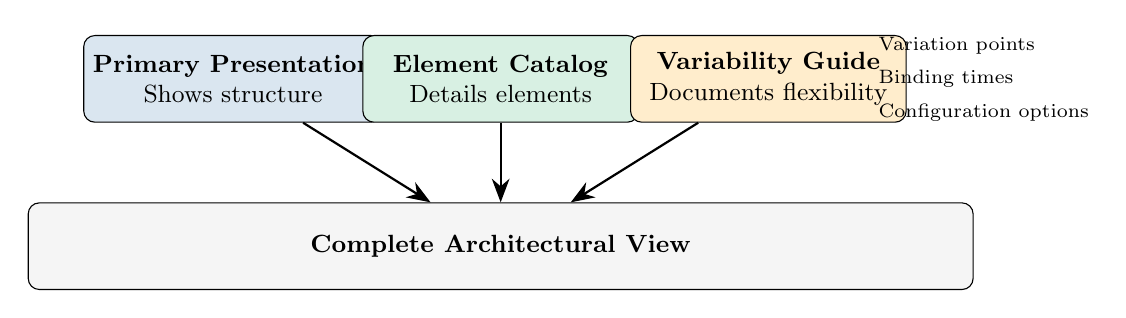
\begin{tikzpicture}[
    scale=0.85,
    box/.style={draw, rounded corners, minimum width=3.5cm, minimum height=1.1cm, align=center, font=\small},
    arrow/.style={-{Stealth[length=3mm]}, thick}
]
    % View components
    \node[box, fill=variationcolor!20] (primary) at (-4,2) {\textbf{Primary Presentation}\\Shows structure};
    \node[box, fill=variantcolor!20] (catalog) at (0,2) {\textbf{Element Catalog}\\Details elements};
    \node[box, fill=bindingcolor!20] (variability) at (4,2) {\textbf{Variability Guide}\\Documents flexibility};
    
    % Complete view
    \node[box, fill=lightgray, minimum width=12cm] (view) at (0,-0.5) {\textbf{Complete Architectural View}};
    
    % Arrows
    \draw[arrow] (primary) -- (view);
    \draw[arrow] (catalog) -- (view);
    \draw[arrow] (variability) -- (view);
    
    % Questions answered
    \node[font=\scriptsize, right] at (5.5,2.5) {Variation points};
    \node[font=\scriptsize, right] at (5.5,2) {Binding times};
    \node[font=\scriptsize, right] at (5.5,1.5) {Configuration options};
\end{tikzpicture}
\caption{Variability Guide within View Documentation}
\end{figure}

\subsection{Standards and Frameworks}

Variability documentation draws from several established approaches. Software Product Line Engineering (SPLE) provides the foundational concepts for systematic variability management. Feature-Oriented Domain Analysis (FODA) introduced feature modeling for representing variability. Common Variability Language (CVL) offers a standardized notation for variability. Orthogonal Variability Model (OVM) provides a view-based approach to variability. ISO/IEC 26550 establishes reference models for software product lines.

%==============================================================================
\section{Variability Concepts and Taxonomy}
%==============================================================================

\subsection{Core Concepts}

Understanding variability requires familiarity with several key concepts.

\begin{definition}
A \textbf{Variation Point} is a location in the architecture where variation can occur---a place where different alternatives (variants) can be selected or configured to customize system behavior or structure.
\end{definition}

\begin{definition}
A \textbf{Variant} is a specific alternative that can be selected at a variation point. Each variant represents one possible way to resolve the variability.
\end{definition}

\begin{definition}
\textbf{Binding Time} is the point in the software lifecycle when a variation point is resolved---when a specific variant is selected and the variability is eliminated.
\end{definition}

\begin{figure}[H]
\centering
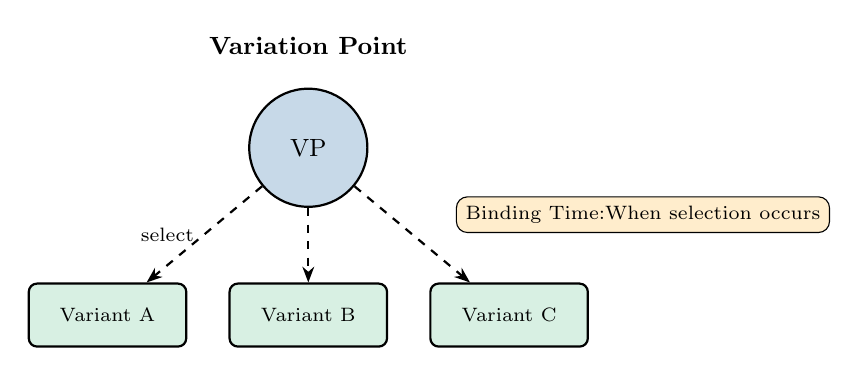
\begin{tikzpicture}[
    scale=0.85,
    vp/.style={draw, thick, fill=variationcolor!30, circle, minimum size=1.5cm, font=\small},
    variant/.style={draw, thick, fill=variantcolor!20, minimum width=2cm, minimum height=0.8cm, rounded corners=3pt, font=\scriptsize},
    arrow/.style={-{Stealth[length=2mm]}, thick}
]
    % Variation point
    \node[vp] (vp) at (0,0) {VP};
    \node[above=0.3cm of vp, font=\small\bfseries] {Variation Point};
    
    % Variants
    \node[variant] (v1) at (-3,-2.5) {Variant A};
    \node[variant] (v2) at (0,-2.5) {Variant B};
    \node[variant] (v3) at (3,-2.5) {Variant C};
    
    % Arrows
    \draw[arrow, dashed] (vp) -- node[left, font=\scriptsize] {select} (v1);
    \draw[arrow, dashed] (vp) -- (v2);
    \draw[arrow, dashed] (vp) -- (v3);
    
    % Binding annotation
    \node[draw, rounded corners, fill=bindingcolor!20, font=\scriptsize] at (5,-1) {Binding Time:\\When selection occurs};
\end{tikzpicture}
\caption{Variation Point, Variants, and Binding}
\end{figure}

\subsection{Types of Variability}

Variability can be classified along several dimensions.

\subsubsection{By Subject}

\begin{longtable}{@{}L{3cm} L{4.5cm} L{5cm}@{}}
\caption{Variability by Subject} \\
\toprule
\textbf{Subject} & \textbf{What Varies} & \textbf{Examples} \\
\midrule
\endfirsthead
\toprule
\textbf{Subject} & \textbf{What Varies} & \textbf{Examples} \\
\midrule
\endhead
\bottomrule
\endlastfoot
Functional & Features and capabilities & Payment methods; report types; workflow steps \\
Data & Data models and schemas & Currency formats; product attributes; user fields \\
Platform & Runtime environment & OS; database; cloud provider \\
Interface & User interaction & Web UI; mobile app; API; CLI \\
Quality & Non-functional properties & Performance tiers; security levels; SLA options \\
Integration & External connections & Third-party APIs; partner systems; protocols \\
Localization & Regional adaptation & Language; date format; currency; regulations \\
\end{longtable}

\subsubsection{By Cardinality}

\begin{longtable}{@{}L{3cm} L{4cm} L{5.5cm}@{}}
\caption{Variability by Cardinality} \\
\toprule
\textbf{Cardinality} & \textbf{Selection Rule} & \textbf{Examples} \\
\midrule
\endfirsthead
\toprule
\textbf{Cardinality} & \textbf{Selection Rule} & \textbf{Examples} \\
\midrule
\endhead
\bottomrule
\endlastfoot
Mandatory & Must be included (no choice) & Core security module; logging \\
Optional & Zero or one selection & Premium features; optional integrations \\
Alternative & Exactly one from set & Database vendor; authentication provider \\
Or & One or more from set & Payment methods; export formats \\
Multiple & Zero or more from set & Plugin modules; add-on features \\
\end{longtable}

\subsubsection{By Visibility}

\begin{longtable}{@{}L{3cm} L{4.5cm} L{5cm}@{}}
\caption{Variability by Visibility} \\
\toprule
\textbf{Visibility} & \textbf{Who Controls} & \textbf{Examples} \\
\midrule
\endfirsthead
\toprule
\textbf{Visibility} & \textbf{Who Controls} & \textbf{Examples} \\
\midrule
\endhead
\bottomrule
\endlastfoot
External & End users or customers & User preferences; tenant settings \\
Product Manager & Product configuration team & Feature toggles; edition definitions \\
Developer & Development team & Build variants; compiler flags \\
Operator & Operations/DevOps team & Deployment parameters; scaling settings \\
Internal & Hidden implementation details & Algorithm selection; optimization strategies \\
\end{longtable}

\subsection{Binding Time Spectrum}

Binding time significantly affects how variability is implemented and managed.

\begin{figure}[H]
\centering
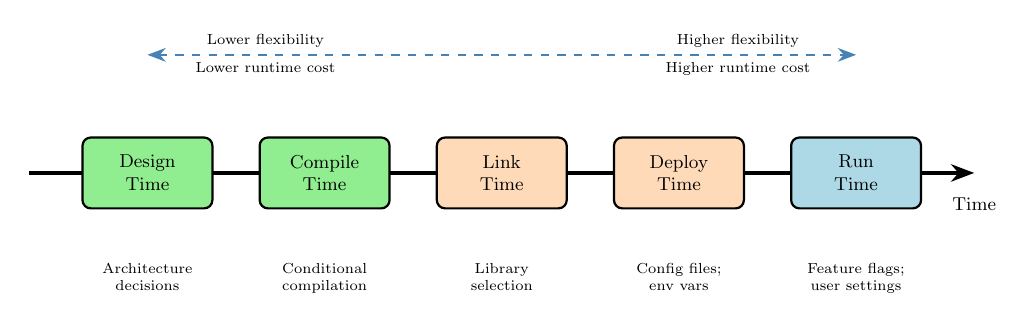
\begin{tikzpicture}[
    scale=0.75,
    transform shape,
    phase/.style={draw, thick, minimum width=2.2cm, minimum height=1.2cm, rounded corners=3pt, font=\small, align=center}
]
    % Timeline
    \draw[-{Stealth}, very thick] (-1,0) -- (15,0);
    \node[below, font=\small] at (15,-0.3) {Time};
    
    % Phases
    \node[phase, fill=compiletime] (design) at (1,0) {Design\\Time};
    \node[phase, fill=compiletime] (compile) at (4,0) {Compile\\Time};
    \node[phase, fill=deploytime] (link) at (7,0) {Link\\Time};
    \node[phase, fill=deploytime] (deploy) at (10,0) {Deploy\\Time};
    \node[phase, fill=runtime] (runtime) at (13,0) {Run\\Time};
    
    % Examples below
    \node[below=0.8cm of design, font=\scriptsize, text width=2cm, align=center] {Architecture decisions};
    \node[below=0.8cm of compile, font=\scriptsize, text width=2cm, align=center] {Conditional compilation};
    \node[below=0.8cm of link, font=\scriptsize, text width=2cm, align=center] {Library selection};
    \node[below=0.8cm of deploy, font=\scriptsize, text width=2cm, align=center] {Config files; env vars};
    \node[below=0.8cm of runtime, font=\scriptsize, text width=2cm, align=center] {Feature flags; user settings};
    
    % Flexibility vs Cost annotation
    \draw[{Stealth}-{Stealth}, thick, dashed, variationcolor] (1,2) -- (13,2);
    \node[above, font=\scriptsize] at (3,2) {Lower flexibility};
    \node[above, font=\scriptsize] at (11,2) {Higher flexibility};
    \node[below, font=\scriptsize] at (3,2) {Lower runtime cost};
    \node[below, font=\scriptsize] at (11,2) {Higher runtime cost};
\end{tikzpicture}
\caption{Binding Time Spectrum with Tradeoffs}
\end{figure}

\subsubsection{Binding Time Details}

\begin{longtable}{@{}L{2.5cm} L{4cm} L{3cm} L{3cm}@{}}
\caption{Binding Time Characteristics} \\
\toprule
\textbf{Binding Time} & \textbf{Mechanism} & \textbf{Advantages} & \textbf{Disadvantages} \\
\midrule
\endfirsthead
\toprule
\textbf{Binding Time} & \textbf{Mechanism} & \textbf{Advantages} & \textbf{Disadvantages} \\
\midrule
\endhead
\bottomrule
\endlastfoot
Design Time & Pattern selection; architecture & Maximum optimization & No flexibility post-design \\
Compile Time & Preprocessor; generics; build profiles & Type safety; optimization & Requires rebuild \\
Link Time & Static/dynamic libraries; DI containers & Modular builds & Deployment per variant \\
Deployment Time & Config files; environment variables & No code changes & Requires redeployment \\
Startup Time & Configuration loading; plugin discovery & Simple management & Requires restart \\
Runtime & Feature flags; settings; A/B tests & Maximum flexibility & Performance overhead \\
\end{longtable}

%==============================================================================
\section{Variation Point Documentation}
%==============================================================================

\subsection{Variation Point Registry}

The variation point registry provides a comprehensive inventory of all points where the architecture supports variation.

\begin{template}
\textbf{Variation Point Specification Template}

\vspace{0.2cm}
\textbf{Identification}
\begin{itemize}[nosep]
    \item \textbf{VP ID:} Unique identifier
    \item \textbf{Name:} Descriptive name
    \item \textbf{Category:} Functional / Data / Platform / Interface / Quality
\end{itemize}

\vspace{0.2cm}
\textbf{Location}
\begin{itemize}[nosep]
    \item \textbf{Element:} Architectural element containing the VP
    \item \textbf{Implementation:} Code/config location
\end{itemize}

\vspace{0.2cm}
\textbf{Variability Characteristics}
\begin{itemize}[nosep]
    \item \textbf{Cardinality:} Mandatory / Optional / Alternative / Or
    \item \textbf{Binding Time:} When variation is resolved
    \item \textbf{Binding Mechanism:} How variation is realized
\end{itemize}

\vspace{0.2cm}
\textbf{Variants}
\begin{itemize}[nosep]
    \item \textbf{Available Variants:} List of options
    \item \textbf{Default:} Default variant if not specified
\end{itemize}

\vspace{0.2cm}
\textbf{Constraints}
\begin{itemize}[nosep]
    \item \textbf{Dependencies:} Required relationships with other VPs
    \item \textbf{Exclusions:} Incompatible combinations
\end{itemize}
\end{template}

\subsection{Comprehensive Variation Point Registry}

\setlength{\extrarowheight}{4pt}
\begin{longtable}{@{}L{1.3cm} L{2.5cm} L{2cm} L{2cm} L{4.2cm}@{}}
\caption{Variation Point Registry} \\
\toprule
\textbf{VP ID} & \textbf{Name} & \textbf{Location} & \textbf{Binding} & \textbf{Description} \\
\midrule
\endfirsthead
\toprule
\textbf{VP ID} & \textbf{Name} & \textbf{Location} & \textbf{Binding} & \textbf{Description} \\
\midrule
\endhead
\midrule
\multicolumn{5}{r}{\textit{Continued on next page}} \\
\endfoot
\bottomrule
\endlastfoot
VP-01 & Database Provider & Data Layer & Deploy & Selection of relational database (PostgreSQL, MySQL, SQL Server) \\
VP-02 & Authentication Method & Auth Service & Deploy & Choice of auth provider (OIDC, SAML, LDAP, Local) \\
VP-03 & Payment Gateway & Checkout & Runtime & Payment processor integration (Stripe, PayPal, Adyen) \\
VP-04 & Search Engine & Catalog & Deploy & Search implementation (Elasticsearch, Algolia, Native) \\
VP-05 & Notification Channels & Notify Service & Runtime & Enabled channels (Email, SMS, Push, Slack) \\
VP-06 & Storage Provider & File Service & Deploy & Object storage (S3, GCS, Azure Blob, MinIO) \\
VP-07 & Cache Strategy & All Services & Deploy & Caching implementation (Redis, Memcached, Local) \\
VP-08 & Feature Flags & All Modules & Runtime & Feature toggle states per environment \\
VP-09 & UI Theme & Frontend & Runtime & Visual theme and branding per tenant \\
VP-10 & Reporting Engine & Analytics & Compile & Report generation (Built-in, Crystal, SSRS) \\
VP-11 & Tax Calculator & Checkout & Runtime & Tax service integration (Avalara, TaxJar, Built-in) \\
VP-12 & Shipping Provider & Fulfillment & Runtime & Carrier integration (FedEx, UPS, DHL, Custom) \\
\end{longtable}

\subsection{Detailed Variation Point Specifications}

\begin{variationbox}[VP-01: Database Provider]

\textbf{Identification}
\begin{itemize}[nosep]
    \item \textbf{ID:} VP-01
    \item \textbf{Name:} Database Provider
    \item \textbf{Category:} Platform
    \item \textbf{Owner:} Platform Team
\end{itemize}

\vspace{0.3cm}
\textbf{Location}
\begin{itemize}[nosep]
    \item \textbf{Element:} Data Access Layer
    \item \textbf{Implementation:} \texttt{config/database.yml}, \texttt{src/data/providers/}
    \item \textbf{View Reference:} [VIEW:DataFlow] Database component
\end{itemize}

\vspace{0.3cm}
\textbf{Variability Characteristics}
\begin{itemize}[nosep]
    \item \textbf{Cardinality:} Alternative (exactly one)
    \item \textbf{Binding Time:} Deployment time
    \item \textbf{Binding Mechanism:} Environment variable + configuration file
    \item \textbf{Rebinding:} Requires redeployment and data migration
\end{itemize}

\vspace{0.3cm}
\textbf{Rationale}

Different deployment environments and customer requirements necessitate support for multiple database vendors. Enterprise customers often mandate specific database vendors for compliance or existing infrastructure alignment. Cloud deployments may prefer managed services from specific providers.

\vspace{0.3cm}
\textbf{Variants}

\begin{tabular}{@{}L{2.5cm} L{4cm} L{5.5cm}@{}}
\toprule
\textbf{Variant} & \textbf{When to Use} & \textbf{Notes} \\
\midrule
PostgreSQL & Default; cloud deployments; new installations & Best feature support; recommended \\
MySQL & Legacy integrations; cost-sensitive deployments & Limited JSON support; avoid for complex queries \\
SQL Server & Enterprise Windows environments & License cost; excellent tooling \\
Aurora & AWS deployments requiring high availability & PostgreSQL-compatible; managed scaling \\
\bottomrule
\end{tabular}

\vspace{0.3cm}
\textbf{Default:} PostgreSQL

\vspace{0.3cm}
\textbf{Configuration}

\begin{lstlisting}[language=bash]
# Environment variable
DATABASE_PROVIDER=postgresql

# config/database.yml
database:
  provider: ${DATABASE_PROVIDER}
  host: ${DB_HOST}
  port: ${DB_PORT}
  name: ${DB_NAME}
  pool_size: 20
\end{lstlisting}

\vspace{0.3cm}
\textbf{Constraints}
\begin{itemize}[nosep]
    \item If \texttt{VP-10 (Reporting Engine) = Crystal Reports}, then \texttt{VP-01 $\neq$ MySQL} (Crystal has MySQL limitations)
    \item Aurora variant requires \texttt{VP-06 (Storage Provider) = S3}
\end{itemize}

\vspace{0.3cm}
\textbf{Quality Impact}
\begin{itemize}[nosep]
    \item \textbf{Performance:} Aurora provides best performance at scale
    \item \textbf{Cost:} MySQL lowest license cost; Aurora highest
    \item \textbf{Portability:} PostgreSQL most portable across cloud providers
\end{itemize}
\end{variationbox}

\begin{variationbox}[VP-03: Payment Gateway]

\textbf{Identification}
\begin{itemize}[nosep]
    \item \textbf{ID:} VP-03
    \item \textbf{Name:} Payment Gateway
    \item \textbf{Category:} Integration
    \item \textbf{Owner:} Payments Team
\end{itemize}

\vspace{0.3cm}
\textbf{Location}
\begin{itemize}[nosep]
    \item \textbf{Element:} Payment Service, Checkout Module
    \item \textbf{Implementation:} \texttt{src/payments/gateways/}, feature flags
    \item \textbf{View Reference:} [VIEW:Component] Payment Service
\end{itemize}

\vspace{0.3cm}
\textbf{Variability Characteristics}
\begin{itemize}[nosep]
    \item \textbf{Cardinality:} Or (one or more from set)
    \item \textbf{Binding Time:} Runtime (per transaction)
    \item \textbf{Binding Mechanism:} Feature flags + customer preferences + availability
    \item \textbf{Rebinding:} Dynamic; no restart required
\end{itemize}

\vspace{0.3cm}
\textbf{Rationale}

Multiple payment gateways provide customer choice, geographic coverage, and redundancy. Customers may prefer specific payment methods. Gateway availability may vary, requiring failover capability. Different gateways offer different fee structures.

\vspace{0.3cm}
\textbf{Variants}

\begin{tabular}{@{}L{2cm} L{3cm} L{3.5cm} L{3.5cm}@{}}
\toprule
\textbf{Variant} & \textbf{Coverage} & \textbf{Strengths} & \textbf{Limitations} \\
\midrule
Stripe & Global & Developer experience; API quality & Higher fees in some regions \\
PayPal & Global & Consumer trust; buyer protection & Lower conversion for some segments \\
Adyen & Global & Enterprise; unified platform & Complex integration \\
Square & US, CA, UK, AU & SMB-focused; POS integration & Limited global coverage \\
\bottomrule
\end{tabular}

\vspace{0.3cm}
\textbf{Default:} Stripe (primary), PayPal (fallback)

\vspace{0.3cm}
\textbf{Selection Logic}

\begin{lstlisting}[language=java]
PaymentGateway selectGateway(Order order, Customer customer) {
    // Customer preference takes priority
    if (customer.preferredGateway != null 
        && isAvailable(customer.preferredGateway)) {
        return customer.preferredGateway;
    }
    
    // Regional optimization
    Gateway regional = getRegionalOptimal(customer.country);
    if (isAvailable(regional)) {
        return regional;
    }
    
    // Fallback chain
    return getFirstAvailable(GATEWAY_PRIORITY_LIST);
}
\end{lstlisting}

\vspace{0.3cm}
\textbf{Constraints}
\begin{itemize}[nosep]
    \item At least one payment gateway must be enabled
    \item Crypto payments (VP-03-Crypto) requires VP-11 (Tax Calculator) $\neq$ Built-in
    \item Square variant requires US, CA, UK, or AU customer location
\end{itemize}

\vspace{0.3cm}
\textbf{Quality Impact}
\begin{itemize}[nosep]
    \item \textbf{Availability:} Multiple gateways increase payment success rate by 5-10\%
    \item \textbf{Performance:} Gateway selection adds 10-20ms latency
    \item \textbf{Cost:} Fee optimization can reduce payment costs by 0.3-0.5\%
\end{itemize}
\end{variationbox}

\begin{variationbox}[VP-08: Feature Flags]

\textbf{Identification}
\begin{itemize}[nosep]
    \item \textbf{ID:} VP-08
    \item \textbf{Name:} Feature Flags
    \item \textbf{Category:} Functional
    \item \textbf{Owner:} Product Team
\end{itemize}

\vspace{0.3cm}
\textbf{Location}
\begin{itemize}[nosep]
    \item \textbf{Element:} All modules (cross-cutting)
    \item \textbf{Implementation:} LaunchDarkly integration, \texttt{src/common/features/}
    \item \textbf{View Reference:} [VIEW:Module] Cross-cutting concerns
\end{itemize}

\vspace{0.3cm}
\textbf{Variability Characteristics}
\begin{itemize}[nosep]
    \item \textbf{Cardinality:} Multiple (independent on/off per flag)
    \item \textbf{Binding Time:} Runtime (instant, per-request)
    \item \textbf{Binding Mechanism:} Feature flag service API
    \item \textbf{Rebinding:} Immediate; no deployment required
\end{itemize}

\vspace{0.3cm}
\textbf{Feature Flag Registry}

\begin{tabular}{@{}L{3cm} L{1.5cm} L{2.5cm} L{5cm}@{}}
\toprule
\textbf{Flag} & \textbf{Default} & \textbf{Scope} & \textbf{Description} \\
\midrule
\texttt{new-checkout-flow} & off & percentage & Redesigned checkout experience \\
\texttt{ai-recommendations} & off & user-segment & ML-powered product recommendations \\
\texttt{crypto-payments} & off & per-tenant & Enable cryptocurrency payments \\
\texttt{dark-mode} & on & per-user & Dark theme option \\
\texttt{beta-features} & off & per-user & Access to beta features \\
\texttt{maintenance-mode} & off & global & System maintenance indicator \\
\bottomrule
\end{tabular}

\vspace{0.3cm}
\textbf{Flag Evaluation Context}

\begin{lstlisting}[language=java]
// Feature flag evaluation with context
boolean isEnabled = featureFlags.evaluate(
    "new-checkout-flow",
    Context.builder()
        .user(currentUser.id)
        .tenant(currentTenant.id)
        .environment(Environment.PRODUCTION)
        .country(currentUser.country)
        .build()
);
\end{lstlisting}

\vspace{0.3cm}
\textbf{Lifecycle Management}
\begin{itemize}[nosep]
    \item New flags start in \texttt{development} environment only
    \item Gradual rollout: 1\% $\rightarrow$ 10\% $\rightarrow$ 50\% $\rightarrow$ 100\%
    \item Flags older than 90 days without changes flagged for review
    \item Permanent flags documented separately from release flags
\end{itemize}
\end{variationbox}

%==============================================================================
\section{Allowed Variants and Selection Rules}
%==============================================================================

\subsection{Variant Documentation Structure}

Each variant should be documented with sufficient detail for selection decisions and implementation.

\begin{template}
\textbf{Variant Specification Template}

\vspace{0.2cm}
\textbf{Identity}
\begin{itemize}[nosep]
    \item \textbf{Variant ID:} Unique identifier
    \item \textbf{Name:} Descriptive name
    \item \textbf{Variation Point:} Parent VP reference
\end{itemize}

\vspace{0.2cm}
\textbf{Description}
\begin{itemize}[nosep]
    \item \textbf{Purpose:} What this variant provides
    \item \textbf{When to Use:} Selection criteria
    \item \textbf{When NOT to Use:} Counter-indications
\end{itemize}

\vspace{0.2cm}
\textbf{Technical Details}
\begin{itemize}[nosep]
    \item \textbf{Implementation:} How it's realized
    \item \textbf{Dependencies:} Required components/libraries
    \item \textbf{Configuration:} Settings required
\end{itemize}

\vspace{0.2cm}
\textbf{Impact Assessment}
\begin{itemize}[nosep]
    \item \textbf{Quality Attributes:} Effects on performance, security, etc.
    \item \textbf{Cost:} Licensing, infrastructure, operational costs
    \item \textbf{Risks:} Known issues or limitations
\end{itemize}
\end{template}

\subsection{Variant Comparison Matrices}

For each variation point with multiple significant variants, provide comparison matrices.

\begin{longtable}{@{}L{2.5cm} C{1.8cm} C{1.8cm} C{1.8cm} C{1.8cm} C{2cm}@{}}
\caption{VP-02: Authentication Method Variants Comparison} \\
\toprule
\textbf{Criterion} & \textbf{OIDC} & \textbf{SAML} & \textbf{LDAP} & \textbf{Local} & \textbf{Weight} \\
\midrule
\endfirsthead
\toprule
\textbf{Criterion} & \textbf{OIDC} & \textbf{SAML} & \textbf{LDAP} & \textbf{Local} & \textbf{Weight} \\
\midrule
\endhead
\bottomrule
\endlastfoot
Modern standard & \checkmark\checkmark & \checkmark & -- & -- & High \\
Enterprise adoption & \checkmark & \checkmark\checkmark & \checkmark\checkmark & -- & High \\
Mobile support & \checkmark\checkmark & \checkmark & -- & \checkmark & Medium \\
Setup complexity & Low & High & Medium & Low & Medium \\
Self-contained & -- & -- & -- & \checkmark\checkmark & Low \\
Federation support & \checkmark\checkmark & \checkmark\checkmark & -- & -- & Medium \\
License cost & Varies & Varies & -- & -- & Medium \\
\midrule
\textbf{Best For} & \multicolumn{2}{l}{Modern SaaS} & \multicolumn{2}{l}{Enterprise} & SMB/Standalone \\
\end{longtable}

\subsection{Selection Decision Trees}

Provide decision trees for complex variant selection.

\begin{figure}[H]
\centering
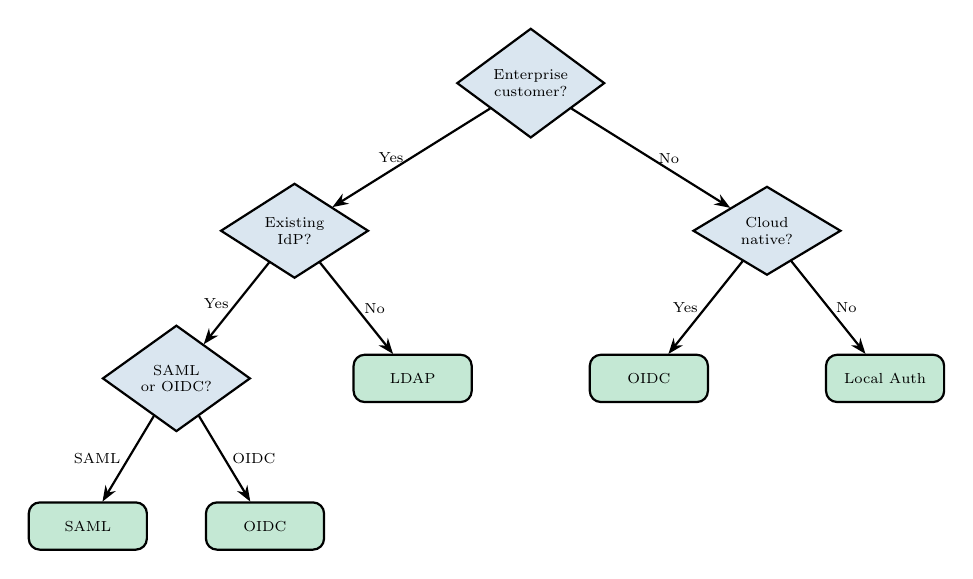
\begin{tikzpicture}[
    scale=0.75,
    transform shape,
    decision/.style={draw, thick, diamond, fill=variationcolor!20, minimum width=2.5cm, minimum height=1.5cm, font=\scriptsize, align=center, inner sep=1pt},
    outcome/.style={draw, thick, fill=variantcolor!30, rounded corners, minimum width=2cm, minimum height=0.8cm, font=\scriptsize},
    arrow/.style={-{Stealth[length=2mm]}, thick}
]
    % Decision nodes
    \node[decision] (d1) at (0,0) {Enterprise\\customer?};
    \node[decision] (d2) at (-4,-2.5) {Existing\\IdP?};
    \node[decision] (d3) at (4,-2.5) {Cloud\\native?};
    \node[decision] (d4) at (-6,-5) {SAML\\or OIDC?};
    
    % Outcomes
    \node[outcome] (ldap) at (-2,-5) {LDAP};
    \node[outcome] (saml) at (-7.5,-7.5) {SAML};
    \node[outcome] (oidc1) at (-4.5,-7.5) {OIDC};
    \node[outcome] (oidc2) at (2,-5) {OIDC};
    \node[outcome] (local) at (6,-5) {Local Auth};
    
    % Arrows
    \draw[arrow] (d1) -- node[left, font=\scriptsize] {Yes} (d2);
    \draw[arrow] (d1) -- node[right, font=\scriptsize] {No} (d3);
    \draw[arrow] (d2) -- node[left, font=\scriptsize] {Yes} (d4);
    \draw[arrow] (d2) -- node[right, font=\scriptsize] {No} (ldap);
    \draw[arrow] (d3) -- node[left, font=\scriptsize] {Yes} (oidc2);
    \draw[arrow] (d3) -- node[right, font=\scriptsize] {No} (local);
    \draw[arrow] (d4) -- node[left, font=\scriptsize] {SAML} (saml);
    \draw[arrow] (d4) -- node[right, font=\scriptsize] {OIDC} (oidc1);
\end{tikzpicture}
\caption{VP-02: Authentication Method Selection Decision Tree}
\end{figure}

\subsection{Variant Selection Rules}

Document formal rules that govern variant selection.

\begin{longtable}{@{}L{1cm} L{3cm} L{5cm} L{3.5cm}@{}}
\caption{Variant Selection Rules} \\
\toprule
\textbf{Rule} & \textbf{Variation Point} & \textbf{Condition} & \textbf{Required Variant} \\
\midrule
\endfirsthead
\toprule
\textbf{Rule} & \textbf{Variation Point} & \textbf{Condition} & \textbf{Required Variant} \\
\midrule
\endhead
\bottomrule
\endlastfoot
SR-01 & VP-01 (Database) & AWS deployment & Aurora or PostgreSQL \\
SR-02 & VP-02 (Auth) & Enterprise tier customer & OIDC or SAML \\
SR-03 & VP-02 (Auth) & Healthcare deployment (HIPAA) & SAML with MFA \\
SR-04 & VP-04 (Search) & Catalog $>$ 100K products & Elasticsearch or Algolia \\
SR-05 & VP-06 (Storage) & Multi-region deployment & S3 or GCS (not MinIO) \\
SR-06 & VP-07 (Cache) & High availability required & Redis with Sentinel \\
SR-07 & VP-11 (Tax) & US customers present & Avalara or TaxJar \\
SR-08 & VP-03 (Payment) & EU customers present & Stripe or Adyen \\
\end{longtable}

%==============================================================================
\section{Configuration Mechanisms}
%==============================================================================

\subsection{Configuration Mechanism Overview}

Different variability types require different configuration mechanisms. The choice of mechanism affects flexibility, safety, and operational complexity.

\begin{figure}[H]
\centering
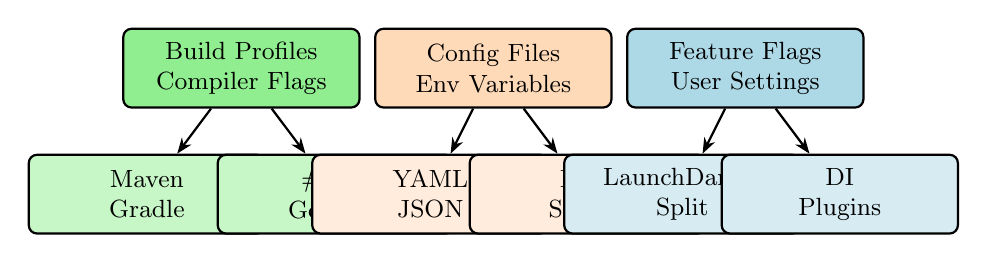
\begin{tikzpicture}[
    scale=0.8,
    mechanism/.style={draw, thick, fill=variationcolor!20, minimum width=3cm, minimum height=1cm, rounded corners=3pt, font=\small, align=center},
    arrow/.style={-{Stealth[length=2mm]}, thick}
]
    % Mechanisms by binding time
    \node[mechanism, fill=compiletime] (compile) at (-4,2) {Build Profiles\\Compiler Flags};
    \node[mechanism, fill=deploytime] (deploy) at (0,2) {Config Files\\Env Variables};
    \node[mechanism, fill=runtime] (runtime) at (4,2) {Feature Flags\\User Settings};
    
    % Implementation technologies
    \node[mechanism, fill=compiletime!50] (maven) at (-5.5,0) {Maven\\Gradle};
    \node[mechanism, fill=compiletime!50] (cpp) at (-2.5,0) {\#ifdef\\Generics};
    
    \node[mechanism, fill=deploytime!50] (yaml) at (-1,0) {YAML\\JSON};
    \node[mechanism, fill=deploytime!50] (env) at (1.5,0) {ENV\\Secrets};
    
    \node[mechanism, fill=runtime!50] (ff) at (3,0) {LaunchDarkly\\Split};
    \node[mechanism, fill=runtime!50] (di) at (5.5,0) {DI\\Plugins};
    
    % Connections
    \draw[arrow] (compile) -- (maven);
    \draw[arrow] (compile) -- (cpp);
    \draw[arrow] (deploy) -- (yaml);
    \draw[arrow] (deploy) -- (env);
    \draw[arrow] (runtime) -- (ff);
    \draw[arrow] (runtime) -- (di);
\end{tikzpicture}
\caption{Configuration Mechanisms by Binding Time}
\end{figure}

\subsection{Configuration Mechanism Catalog}

\begin{longtable}{@{}L{2.5cm} L{2.5cm} L{3.5cm} L{4cm}@{}}
\caption{Configuration Mechanism Catalog} \\
\toprule
\textbf{Mechanism} & \textbf{Binding Time} & \textbf{Use Cases} & \textbf{Implementation} \\
\midrule
\endfirsthead
\toprule
\textbf{Mechanism} & \textbf{Binding Time} & \textbf{Use Cases} & \textbf{Implementation} \\
\midrule
\endhead
\bottomrule
\endlastfoot
Build Profiles & Compile & Platform variants; optional modules & Maven/Gradle profiles \\
Conditional Compilation & Compile & Platform-specific code; debug code & Preprocessor; annotations \\
Dependency Injection & Startup & Service implementations; strategies & Spring; Guice; CDI \\
Configuration Files & Deploy/Startup & Environment settings; credentials & YAML; JSON; Properties \\
Environment Variables & Deploy & Container config; secrets & Docker ENV; K8s ConfigMaps \\
Feature Flags & Runtime & Gradual rollout; A/B testing & LaunchDarkly; Split; Flagsmith \\
Plugin Architecture & Runtime & Extensions; integrations & OSGi; SPI; Module systems \\
User Preferences & Runtime & Personalization; UI settings & Database; local storage \\
Tenant Configuration & Runtime & Multi-tenant customization & Database per tenant \\
Dynamic Discovery & Runtime & Service instances; resources & Consul; Eureka; K8s Services \\
\end{longtable}

\subsection{Configuration File Specifications}

\begin{configbox}[Primary Configuration: application.yml]

\textbf{Purpose:} Central configuration for deployment-time variability

\textbf{Location:} \texttt{config/application.yml}, overridden by environment-specific files

\begin{lstlisting}[language=yaml]
# Application Configuration Schema
app:
  name: ecommerce-platform
  environment: ${APP_ENV:development}
  
# VP-01: Database Provider
database:
  provider: ${DB_PROVIDER:postgresql}  # postgresql, mysql, sqlserver
  host: ${DB_HOST:localhost}
  port: ${DB_PORT:5432}
  name: ${DB_NAME:ecommerce}
  pool:
    min: ${DB_POOL_MIN:5}
    max: ${DB_POOL_MAX:20}
    
# VP-02: Authentication Method
auth:
  provider: ${AUTH_PROVIDER:oidc}  # oidc, saml, ldap, local
  oidc:
    issuer: ${OIDC_ISSUER}
    client-id: ${OIDC_CLIENT_ID}
    client-secret: ${OIDC_CLIENT_SECRET}
  saml:
    metadata-url: ${SAML_METADATA_URL}
    entity-id: ${SAML_ENTITY_ID}
    
# VP-04: Search Engine
search:
  provider: ${SEARCH_PROVIDER:elasticsearch}
  elasticsearch:
    hosts: ${ES_HOSTS:localhost:9200}
    index-prefix: ${ES_INDEX_PREFIX:ecom}
  algolia:
    app-id: ${ALGOLIA_APP_ID}
    api-key: ${ALGOLIA_API_KEY}
    
# VP-07: Cache Strategy
cache:
  provider: ${CACHE_PROVIDER:redis}
  redis:
    host: ${REDIS_HOST:localhost}
    port: ${REDIS_PORT:6379}
    ttl-seconds: ${CACHE_TTL:3600}
    
# VP-05: Notification Channels (multi-select)
notifications:
  channels:
    email:
      enabled: ${NOTIFY_EMAIL_ENABLED:true}
      provider: ${EMAIL_PROVIDER:sendgrid}
    sms:
      enabled: ${NOTIFY_SMS_ENABLED:false}
      provider: ${SMS_PROVIDER:twilio}
    push:
      enabled: ${NOTIFY_PUSH_ENABLED:true}
      provider: ${PUSH_PROVIDER:firebase}
\end{lstlisting}

\textbf{Environment Overrides:}
\begin{itemize}[nosep]
    \item \texttt{application-development.yml} -- Local development defaults
    \item \texttt{application-staging.yml} -- Staging environment
    \item \texttt{application-production.yml} -- Production settings
\end{itemize}

\textbf{Secret Management:}
\begin{itemize}[nosep]
    \item Secrets stored in AWS Secrets Manager / HashiCorp Vault
    \item Referenced via environment variables, not in config files
    \item Rotated according to security policy
\end{itemize}
\end{configbox}

\subsection{Feature Flag Configuration}

\begin{configbox}[Feature Flag Configuration]

\textbf{Purpose:} Runtime variability for gradual rollout and experimentation

\textbf{Provider:} LaunchDarkly

\begin{lstlisting}[language=yaml]
# Feature Flag Definitions (feature-flags.yml)
flags:
  new-checkout-flow:
    key: new-checkout-flow
    name: "New Checkout Experience"
    description: "Redesigned checkout with fewer steps"
    type: boolean
    default: false
    targeting:
      - environment: production
        rules:
          - percentage: 10  # 10% of users
          - segments: [beta-testers]  # All beta testers
      - environment: staging
        default: true  # Always on in staging
    metrics:
      - conversion-rate
      - checkout-completion-time
      
  ai-recommendations:
    key: ai-recommendations
    name: "AI Product Recommendations"
    description: "ML-powered product recommendations"
    type: boolean
    default: false
    targeting:
      - environment: production
        rules:
          - segments: [premium-tier]  # Premium customers only
    prerequisites:
      - flag: data-collection-consent
        value: true
    
  payment-methods:
    key: payment-methods
    name: "Enabled Payment Methods"
    description: "Available payment options"
    type: multivariate
    variants:
      - value: [stripe, paypal]
        name: "Standard"
      - value: [stripe, paypal, crypto]
        name: "With Crypto"
      - value: [stripe, paypal, affirm]
        name: "With BNPL"
    default: [stripe, paypal]
\end{lstlisting}

\textbf{Flag Evaluation Code:}
\begin{lstlisting}[language=java]
@Service
public class FeatureFlagService {
    private final LDClient ldClient;
    
    public boolean isEnabled(String flagKey, User user) {
        LDContext context = LDContext.builder(user.getId())
            .set("email", user.getEmail())
            .set("tier", user.getSubscriptionTier())
            .set("country", user.getCountry())
            .build();
            
        return ldClient.boolVariation(flagKey, context, false);
    }
    
    public List<String> getPaymentMethods(User user) {
        LDContext context = buildContext(user);
        LDValue value = ldClient.jsonValueVariation(
            "payment-methods", context, 
            LDValue.parse("[\"stripe\", \"paypal\"]")
        );
        return parsePaymentMethods(value);
    }
}
\end{lstlisting}
\end{configbox}

\subsection{Plugin and Extension Mechanism}

\begin{configbox}[Plugin Architecture]

\textbf{Purpose:} Extensibility for custom integrations and third-party extensions

\textbf{Mechanism:} Java SPI (Service Provider Interface) + Spring auto-configuration

\begin{lstlisting}[language=java]
// Plugin interface definition
public interface PaymentGatewayPlugin {
    String getGatewayId();
    String getDisplayName();
    boolean supportsCountry(String countryCode);
    PaymentResult processPayment(PaymentRequest request);
    RefundResult processRefund(RefundRequest request);
}

// Plugin registration (META-INF/services)
// File: META-INF/services/com.platform.PaymentGatewayPlugin
com.stripe.StripePaymentGateway
com.paypal.PayPalPaymentGateway
com.custom.CustomPaymentGateway

// Plugin discovery and loading
@Configuration
public class PaymentGatewayConfiguration {
    @Bean
    public PaymentGatewayRegistry gatewayRegistry() {
        ServiceLoader<PaymentGatewayPlugin> loader = 
            ServiceLoader.load(PaymentGatewayPlugin.class);
        
        PaymentGatewayRegistry registry = new PaymentGatewayRegistry();
        for (PaymentGatewayPlugin plugin : loader) {
            registry.register(plugin.getGatewayId(), plugin);
            log.info("Registered payment gateway: {}", 
                     plugin.getDisplayName());
        }
        return registry;
    }
}
\end{lstlisting}

\textbf{Plugin Discovery Locations:}
\begin{itemize}[nosep]
    \item \texttt{/plugins/} directory scanned at startup
    \item Maven/Gradle dependencies with \texttt{@AutoConfiguration}
    \item Database-registered plugins for runtime loading
\end{itemize}

\textbf{Plugin Lifecycle:}
\begin{enumerate}[nosep]
    \item Discovery: Plugins found via SPI or classpath scanning
    \item Validation: Plugin compatibility and security verification
    \item Registration: Plugin added to registry
    \item Activation: Plugin enabled via configuration
    \item Monitoring: Plugin health and usage tracked
\end{enumerate}
\end{configbox}

%==============================================================================
\section{Constraints and Invariants}
%==============================================================================

\subsection{Constraint Types}

Constraints restrict which combinations of variants are valid. Proper constraint documentation prevents invalid configurations.

\begin{longtable}{@{}L{3cm} L{4.5cm} L{5cm}@{}}
\caption{Constraint Types} \\
\toprule
\textbf{Type} & \textbf{Description} & \textbf{Example} \\
\midrule
\endfirsthead
\toprule
\textbf{Type} & \textbf{Description} & \textbf{Example} \\
\midrule
\endhead
\bottomrule
\endlastfoot
Requires & One variant requires another & Crypto payments requires non-built-in tax calculator \\
Excludes & Two variants cannot coexist & LDAP auth excludes OAuth social login \\
Implies & Selecting one implies another & Enterprise tier implies OIDC or SAML auth \\
Cardinality & Limits on number of selections & Maximum 3 payment gateways active \\
Conditional & Context-dependent constraints & AWS deployment requires S3 storage \\
Temporal & Time-based constraints & Cannot change database provider mid-contract \\
\end{longtable}

\subsection{Constraint Specification}

\begin{longtable}{@{}L{1.3cm} L{2.5cm} L{3cm} L{5.5cm}@{}}
\caption{Configuration Constraints Registry} \\
\toprule
\textbf{ID} & \textbf{Type} & \textbf{Constraint} & \textbf{Rationale / Validation} \\
\midrule
\endfirsthead
\toprule
\textbf{ID} & \textbf{Type} & \textbf{Constraint} & \textbf{Rationale / Validation} \\
\midrule
\endhead
\midrule
\multicolumn{4}{r}{\textit{Continued on next page}} \\
\endfoot
\bottomrule
\endlastfoot
CON-01 & Requires & VP-03.Crypto $\rightarrow$ VP-11 $\neq$ BuiltIn & Crypto requires proper tax calculation for regulatory compliance \\
CON-02 & Excludes & VP-02.LDAP $\times$ VP-02.SocialLogin & LDAP enterprise environments typically prohibit social login \\
CON-03 & Implies & Enterprise Tier $\rightarrow$ VP-02 $\in$ \{OIDC, SAML\} & Enterprise customers require SSO integration \\
CON-04 & Cardinality & $|$VP-03 selections$|$ $\leq$ 3 & Performance and maintenance limits \\
CON-05 & Conditional & AWS $\rightarrow$ VP-06 $\in$ \{S3, Aurora\} & AWS deployment optimized for AWS services \\
CON-06 & Requires & VP-04.Algolia $\rightarrow$ VP-07.Redis & Algolia sync requires Redis for queue management \\
CON-07 & Excludes & VP-01.MySQL $\times$ VP-10.Crystal & Crystal Reports has known MySQL compatibility issues \\
CON-08 & Requires & VP-08.AiRecommendations $\rightarrow$ DataConsent=true & ML features require data collection consent \\
CON-09 & Cardinality & $|$VP-05 selections$|$ $\geq$ 1 & At least one notification channel required \\
CON-10 & Temporal & VP-01 cannot change during contract & Database migration disruptive; plan at renewal \\
\end{longtable}

\subsection{Constraint Visualization}

\begin{figure}[H]
\centering
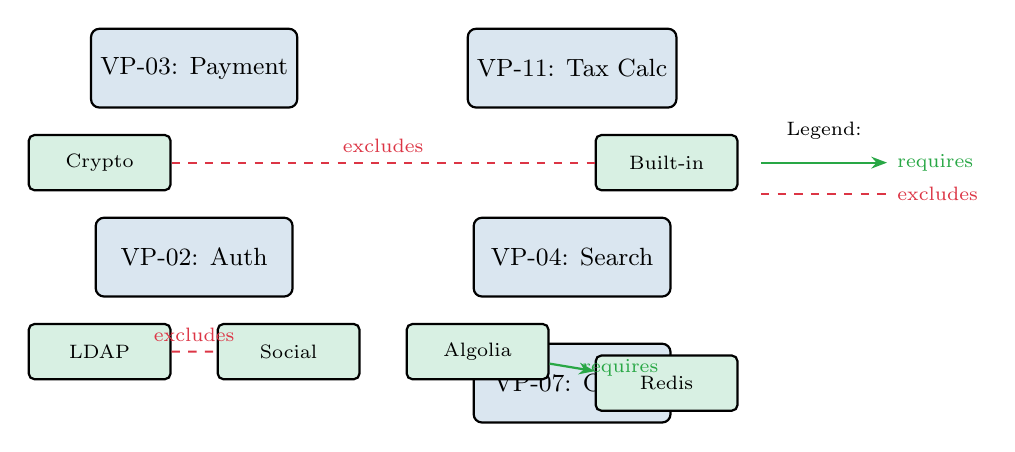
\begin{tikzpicture}[
    scale=0.8,
    vp/.style={draw, thick, fill=variationcolor!20, minimum width=2.5cm, minimum height=1cm, rounded corners=3pt, font=\small},
    variant/.style={draw, thick, fill=variantcolor!20, minimum width=1.8cm, minimum height=0.7cm, rounded corners=2pt, font=\scriptsize},
    requires/.style={-{Stealth[length=2mm]}, thick, successgreen},
    excludes/.style={thick, warningred, dashed}
]
    % Variation Points
    \node[vp] (payment) at (0,3) {VP-03: Payment};
    \node[vp] (tax) at (6,3) {VP-11: Tax Calc};
    \node[vp] (auth) at (0,0) {VP-02: Auth};
    \node[vp] (search) at (6,0) {VP-04: Search};
    \node[vp] (cache) at (6,-2) {VP-07: Cache};
    
    % Variants
    \node[variant] (crypto) at (-1.5,1.5) {Crypto};
    \node[variant] (builtin) at (7.5,1.5) {Built-in};
    \node[variant] (ldap) at (-1.5,-1.5) {LDAP};
    \node[variant] (social) at (1.5,-1.5) {Social};
    \node[variant] (algolia) at (4.5,-1.5) {Algolia};
    \node[variant] (redis) at (7.5,-2) {Redis};
    
    % Constraints
    \draw[excludes] (crypto) -- node[above, font=\scriptsize, sloped] {excludes} (builtin);
    \draw[excludes] (ldap) -- node[above, font=\scriptsize] {excludes} (social);
    \draw[requires] (algolia) -- node[right, font=\scriptsize] {requires} (redis);
    
    % Legend
    \node[font=\scriptsize] at (10,2) {Legend:};
    \draw[requires] (9,1.5) -- (11,1.5) node[right, font=\scriptsize] {requires};
    \draw[excludes] (9,1) -- (11,1) node[right, font=\scriptsize] {excludes};
\end{tikzpicture}
\caption{Constraint Relationships Visualization}
\end{figure}

\subsection{Constraint Validation}

\begin{lstlisting}[language=java, caption=Configuration Validation Implementation]
@Component
public class ConfigurationValidator {
    
    public ValidationResult validate(SystemConfiguration config) {
        List<ConstraintViolation> violations = new ArrayList<>();
        
        // CON-01: Crypto requires non-built-in tax
        if (config.paymentGateways.contains("crypto") 
            && config.taxCalculator.equals("builtin")) {
            violations.add(new ConstraintViolation("CON-01",
                "Crypto payments require external tax calculator"));
        }
        
        // CON-02: LDAP excludes social login
        if (config.authProvider.equals("ldap") 
            && config.socialLoginEnabled) {
            violations.add(new ConstraintViolation("CON-02",
                "LDAP auth is incompatible with social login"));
        }
        
        // CON-04: Max 3 payment gateways
        if (config.paymentGateways.size() > 3) {
            violations.add(new ConstraintViolation("CON-04",
                "Maximum 3 payment gateways allowed"));
        }
        
        // CON-06: Algolia requires Redis
        if (config.searchProvider.equals("algolia") 
            && !config.cacheProvider.equals("redis")) {
            violations.add(new ConstraintViolation("CON-06",
                "Algolia search requires Redis cache"));
        }
        
        return new ValidationResult(violations);
    }
}
\end{lstlisting}

%==============================================================================
\section{Configuration Examples and Scenarios}
%==============================================================================

\subsection{Product Configuration Profiles}

Define standard configuration profiles for common deployment scenarios.

\begin{variationbox}[Configuration Profile: Startup Edition]

\textbf{Target:} Small businesses, startups, individual sellers

\textbf{Characteristics:} Low cost, simple setup, limited scale

\vspace{0.3cm}
\textbf{Variation Point Selections:}

\begin{tabular}{@{}L{4cm} L{4cm} L{4.5cm}@{}}
\toprule
\textbf{Variation Point} & \textbf{Selected Variant} & \textbf{Rationale} \\
\midrule
VP-01: Database & PostgreSQL (shared) & Cost-effective; sufficient for scale \\
VP-02: Authentication & Local Auth & Simple; no SSO needed \\
VP-03: Payment Gateway & Stripe only & Single provider; lower complexity \\
VP-04: Search & Native (built-in) & Adequate for small catalogs \\
VP-05: Notifications & Email only & Basic notifications sufficient \\
VP-06: Storage & S3 (shared bucket) & Cost-effective object storage \\
VP-07: Cache & Local (in-memory) & Sufficient for single instance \\
VP-08: Feature Flags & Basic set only & Limited feature set \\
VP-11: Tax Calculator & Built-in (US only) & Simple tax rules \\
\bottomrule
\end{tabular}

\vspace{0.3cm}
\textbf{Infrastructure:}
\begin{itemize}[nosep]
    \item Single application instance
    \item Shared PostgreSQL database
    \item Shared S3 bucket with tenant prefix
    \item No Redis required
\end{itemize}

\textbf{Limitations:}
\begin{itemize}[nosep]
    \item Maximum 10,000 products
    \item Maximum 1,000 orders/day
    \item US market only (tax limitation)
    \item No SSO integration
\end{itemize}

\textbf{Configuration File:}
\begin{lstlisting}[language=yaml]
edition: startup
database:
  provider: postgresql
  multi-tenant: shared
auth:
  provider: local
payment:
  gateways: [stripe]
search:
  provider: native
\end{lstlisting}
\end{variationbox}

\begin{variationbox}[Configuration Profile: Enterprise Edition]

\textbf{Target:} Large enterprises, high-volume retailers

\textbf{Characteristics:} High scale, full features, enterprise integration

\vspace{0.3cm}
\textbf{Variation Point Selections:}

\begin{tabular}{@{}L{4cm} L{4cm} L{4.5cm}@{}}
\toprule
\textbf{Variation Point} & \textbf{Selected Variant} & \textbf{Rationale} \\
\midrule
VP-01: Database & Aurora (dedicated) & High availability; auto-scaling \\
VP-02: Authentication & SAML + OIDC & Enterprise SSO integration \\
VP-03: Payment Gateway & Stripe + PayPal + Adyen & Global coverage; redundancy \\
VP-04: Search & Elasticsearch (dedicated) & High-volume catalog support \\
VP-05: Notifications & All channels & Full communication capability \\
VP-06: Storage & S3 (dedicated bucket) & Isolation; compliance \\
VP-07: Cache & Redis Cluster & High availability caching \\
VP-08: Feature Flags & Full access + custom & All features; A/B testing \\
VP-11: Tax Calculator & Avalara & Global tax compliance \\
\bottomrule
\end{tabular}

\vspace{0.3cm}
\textbf{Infrastructure:}
\begin{itemize}[nosep]
    \item Multi-AZ deployment (3+ instances)
    \item Dedicated Aurora cluster with read replicas
    \item Dedicated Elasticsearch cluster
    \item Redis Cluster with 6 nodes
    \item Dedicated S3 bucket with encryption
\end{itemize}

\textbf{Capabilities:}
\begin{itemize}[nosep]
    \item Unlimited products
    \item 100,000+ orders/day
    \item Global market support
    \item Full SSO integration
    \item 99.95\% SLA
\end{itemize}

\textbf{Configuration File:}
\begin{lstlisting}[language=yaml]
edition: enterprise
database:
  provider: aurora
  multi-tenant: dedicated
  replicas: 2
auth:
  provider: saml
  fallback: oidc
  mfa: required
payment:
  gateways: [stripe, paypal, adyen]
  failover: true
search:
  provider: elasticsearch
  cluster-size: 3
cache:
  provider: redis
  cluster: true
  nodes: 6
\end{lstlisting}
\end{variationbox}

\subsection{Migration Scenarios}

Document how to transition between configurations.

\begin{example}
\textbf{Migration Scenario: Startup to Professional Edition}

\textbf{Trigger:} Customer exceeds 10,000 products or 1,000 orders/day

\textbf{Changes Required:}
\begin{enumerate}[nosep]
    \item VP-01: Migrate from shared to dedicated PostgreSQL
    \item VP-04: Migrate from native search to Elasticsearch
    \item VP-07: Add Redis cache layer
    \item VP-03: Add PayPal as second payment option
\end{enumerate}

\textbf{Migration Steps:}
\begin{enumerate}
    \item Provision dedicated PostgreSQL instance
    \item Replicate data from shared database
    \item Deploy Elasticsearch and index catalog
    \item Update configuration to point to new services
    \item Enable Redis cache
    \item Switch traffic to new configuration
    \item Verify functionality
    \item Decommission shared resources
\end{enumerate}

\textbf{Downtime:} Zero (blue-green deployment)

\textbf{Duration:} 2-4 hours (automated)

\textbf{Rollback:} Revert DNS; maintain old configuration for 24 hours
\end{example}

%==============================================================================
\section{Traceability}
%==============================================================================

\subsection{Variability to Requirements Traceability}

\begin{longtable}{@{}L{2cm} L{5.5cm} L{5cm}@{}}
\caption{Variation Points to Requirements Mapping} \\
\toprule
\textbf{VP ID} & \textbf{Requirements} & \textbf{Features/Capabilities} \\
\midrule
\endfirsthead
\toprule
\textbf{VP ID} & \textbf{Requirements} & \textbf{Features/Capabilities} \\
\midrule
\endhead
\bottomrule
\endlastfoot
VP-01 & REQ-NFR-001 (Performance), REQ-NFR-003 (Scalability) & Platform flexibility \\
VP-02 & REQ-SEC-001 (Authentication), REQ-SEC-005 (SSO) & Enterprise SSO, Security \\
VP-03 & REQ-FUNC-042 (Payments), REQ-FUNC-045 (Multi-currency) & Payment processing \\
VP-04 & REQ-FUNC-010 (Product Search), REQ-NFR-002 (Search Performance) & Catalog search \\
VP-05 & REQ-FUNC-060 (Notifications), REQ-FUNC-062 (Multi-channel) & Customer communication \\
VP-08 & REQ-OPS-010 (Feature Control), REQ-PROD-001 (A/B Testing) & Release management \\
VP-11 & REQ-COMPL-001 (Tax Compliance), REQ-FUNC-050 (Tax Calculation) & Tax handling \\
\end{longtable}

\subsection{Variability to Implementation Traceability}

\begin{longtable}{@{}L{1.5cm} L{4.5cm} L{3cm} L{3.5cm}@{}}
\caption{Variation Points to Implementation Mapping} \\
\toprule
\textbf{VP ID} & \textbf{Implementation Artifacts} & \textbf{Configuration} & \textbf{Tests} \\
\midrule
\endfirsthead
\toprule
\textbf{VP ID} & \textbf{Implementation Artifacts} & \textbf{Configuration} & \textbf{Tests} \\
\midrule
\endhead
\bottomrule
\endlastfoot
VP-01 & \texttt{src/data/providers/} & \texttt{database.*} & \texttt{DatabaseProviderTest} \\
VP-02 & \texttt{src/auth/providers/} & \texttt{auth.*} & \texttt{AuthIntegrationTest} \\
VP-03 & \texttt{src/payments/gateways/} & \texttt{payment.gateways} & \texttt{PaymentGatewayTest} \\
VP-04 & \texttt{src/search/engines/} & \texttt{search.*} & \texttt{SearchEngineTest} \\
VP-07 & \texttt{src/cache/providers/} & \texttt{cache.*} & \texttt{CacheProviderTest} \\
VP-08 & \texttt{src/common/features/} & LaunchDarkly & \texttt{FeatureFlagTest} \\
\end{longtable}

\subsection{Variability to Deployment Traceability}

\begin{longtable}{@{}L{1.5cm} L{3.5cm} L{4cm} L{3.5cm}@{}}
\caption{Variation Points to Deployment Mapping} \\
\toprule
\textbf{VP ID} & \textbf{Infrastructure} & \textbf{Kubernetes Resources} & \textbf{Monitoring} \\
\midrule
\endfirsthead
\toprule
\textbf{VP ID} & \textbf{Infrastructure} & \textbf{Kubernetes Resources} & \textbf{Monitoring} \\
\midrule
\endhead
\bottomrule
\endlastfoot
VP-01 & RDS / Aurora / CloudSQL & \texttt{database-secret} & DB connection metrics \\
VP-02 & Identity provider & \texttt{auth-config} & Auth success/failure rates \\
VP-03 & Payment gateway accounts & \texttt{payment-secrets} & Transaction success rates \\
VP-04 & Elasticsearch cluster & \texttt{search-config} & Search latency, indexing \\
VP-06 & S3 / GCS bucket & \texttt{storage-secret} & Storage usage, latency \\
VP-07 & Redis cluster & \texttt{redis-config} & Cache hit rates, memory \\
\end{longtable}

%==============================================================================
\section{Variability Governance}
%==============================================================================

\subsection{Variability Management Process}

\begin{figure}[H]
\centering
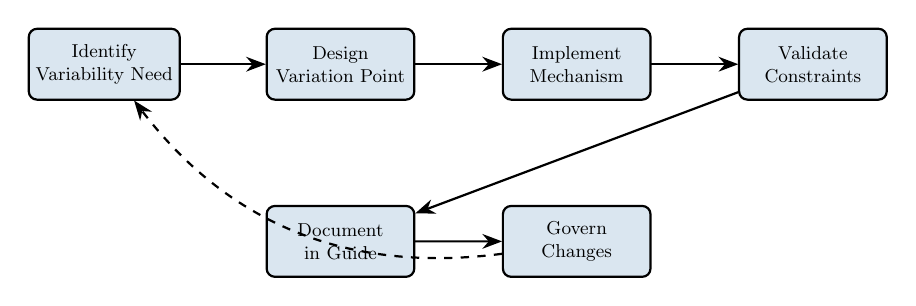
\begin{tikzpicture}[
    scale=0.75,
    transform shape,
    phase/.style={draw, thick, fill=variationcolor!20, minimum width=2.5cm, minimum height=1.2cm, rounded corners=3pt, font=\small, align=center},
    arrow/.style={-{Stealth[length=2.5mm]}, thick}
]
    % Phases
    \node[phase] (identify) at (0,0) {Identify\\Variability Need};
    \node[phase] (design) at (4,0) {Design\\Variation Point};
    \node[phase] (implement) at (8,0) {Implement\\Mechanism};
    \node[phase] (validate) at (12,0) {Validate\\Constraints};
    \node[phase] (document) at (4,-3) {Document\\in Guide};
    \node[phase] (govern) at (8,-3) {Govern\\Changes};
    
    % Arrows
    \draw[arrow] (identify) -- (design);
    \draw[arrow] (design) -- (implement);
    \draw[arrow] (implement) -- (validate);
    \draw[arrow] (validate) -- (document);
    \draw[arrow] (document) -- (govern);
    \draw[arrow, dashed] (govern) to[bend left=30] (identify);
\end{tikzpicture}
\caption{Variability Management Lifecycle}
\end{figure}

\subsection{Change Management for Variability}

\begin{longtable}{@{}L{3cm} L{3.5cm} L{3cm} L{3cm}@{}}
\caption{Variability Change Categories} \\
\toprule
\textbf{Change Type} & \textbf{Examples} & \textbf{Approval} & \textbf{Impact} \\
\midrule
\endfirsthead
\toprule
\textbf{Change Type} & \textbf{Examples} & \textbf{Approval} & \textbf{Impact} \\
\midrule
\endhead
\bottomrule
\endlastfoot
Add Variant & New payment gateway & Tech Lead & Low \\
Remove Variant & Deprecate old provider & Architecture Board & Medium \\
Add VP & New variation point & Architecture Board & High \\
Remove VP & Eliminate variability & Architecture Board & High \\
Modify Constraint & Change compatibility rules & Tech Lead & Medium \\
Change Binding Time & Move from deploy to runtime & Architecture Board & High \\
\end{longtable}

\subsection{Version History}

\begin{longtable}{@{}L{1.5cm} L{2cm} L{2.5cm} L{6.5cm}@{}}
\caption{Variability Guide Version History} \\
\toprule
\textbf{Version} & \textbf{Date} & \textbf{Author} & \textbf{Changes} \\
\midrule
\endfirsthead
\toprule
\textbf{Version} & \textbf{Date} & \textbf{Author} & \textbf{Changes} \\
\midrule
\endhead
\bottomrule
\endlastfoot
1.0.0 & 2024-01-15 & Platform Team & Initial variability guide \\
1.1.0 & 2024-02-20 & J. Smith & Added VP-08 (Feature Flags) \\
1.2.0 & 2024-03-15 & A. Jones & Added Crypto payment variant to VP-03 \\
1.3.0 & 2024-04-10 & Platform Team & Added Enterprise configuration profile \\
2.0.0 & 2024-06-01 & Architecture Team & Major revision; added constraint validation \\
\end{longtable}

%==============================================================================
\section{Open Issues and Future Variability}
%==============================================================================

\subsection{Pending Variability Decisions}

\begin{longtable}{@{}L{1cm} L{4cm} L{2.5cm} L{2.5cm} L{2.5cm}@{}}
\caption{Pending Variability Issues} \\
\toprule
\textbf{ID} & \textbf{Issue} & \textbf{Impact} & \textbf{Target Date} & \textbf{Owner} \\
\midrule
\endfirsthead
\toprule
\textbf{ID} & \textbf{Issue} & \textbf{Impact} & \textbf{Target Date} & \textbf{Owner} \\
\midrule
\endhead
\bottomrule
\endlastfoot
OI-01 & GraphQL API variant needed? & New VP required & Q3 2024 & API Team \\
OI-02 & Multi-region deployment variants & VP-01, VP-06, VP-07 affected & Q4 2024 & Platform \\
OI-03 & Mobile SDK variability & May need new VPs & Q3 2024 & Mobile Team \\
OI-04 & White-label customization depth & UI variability scope & Q2 2024 & Product \\
\end{longtable}

\subsection{Planned Variability Extensions}

\begin{longtable}{@{}L{3cm} L{4cm} L{3cm} L{2.5cm}@{}}
\caption{Planned Variability Additions} \\
\toprule
\textbf{Variation Point} & \textbf{Description} & \textbf{Variants Planned} & \textbf{Timeline} \\
\midrule
\endfirsthead
\toprule
\textbf{Variation Point} & \textbf{Description} & \textbf{Variants Planned} & \textbf{Timeline} \\
\midrule
\endhead
\bottomrule
\endlastfoot
VP-13: CDN Provider & Content delivery network selection & CloudFront, Cloudflare, Fastly & Q3 2024 \\
VP-14: ML Platform & Machine learning infrastructure & SageMaker, Vertex AI, Self-hosted & Q4 2024 \\
VP-15: Workflow Engine & Business process automation & Temporal, Camunda, Built-in & Q4 2024 \\
\end{longtable}

%==============================================================================
\section{Appendix A: Feature Model Notation}
%==============================================================================

\begin{figure}[H]
\centering
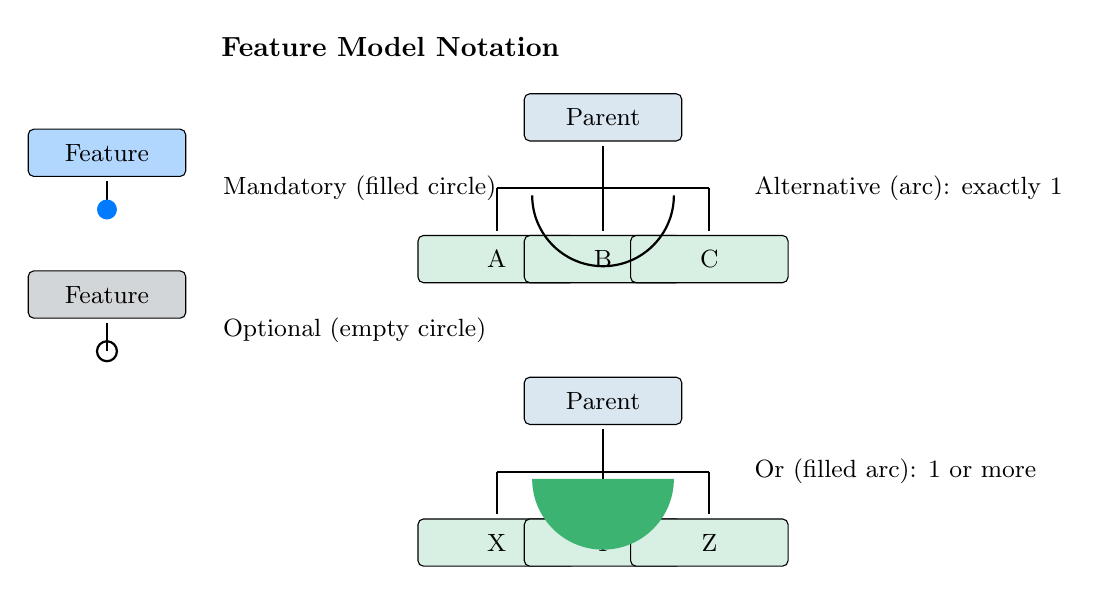
\begin{tikzpicture}[
    scale=0.9,
    feature/.style={draw, minimum width=2cm, minimum height=0.6cm, rounded corners=2pt, font=\small},
    arrow/.style={-, thick}
]
    % Legend
    \node[font=\bfseries] at (0,5) {Feature Model Notation};
    
    % Mandatory
    \node[feature, fill=mandatorycolor!30] at (-4,3.5) {Feature};
    \draw[thick] (-4,3.1) -- (-4,2.7);
    \fill[mandatorycolor] (-4,2.7) circle (4pt);
    \node[right, font=\small] at (-2.5,3) {Mandatory (filled circle)};
    
    % Optional
    \node[feature, fill=optionalcolor!30] at (-4,1.5) {Feature};
    \draw[thick] (-4,1.1) -- (-4,0.7);
    \draw[thick] (-4,0.7) circle (4pt);
    \node[right, font=\small] at (-2.5,1) {Optional (empty circle)};
    
    % Alternative (XOR)
    \node[feature, fill=variationcolor!20] at (3,4) {Parent};
    \node[feature, fill=variantcolor!20] at (1.5,2) {A};
    \node[feature, fill=variantcolor!20] at (3,2) {B};
    \node[feature, fill=variantcolor!20] at (4.5,2) {C};
    \draw[thick] (3,3.6) -- (3,3);
    \draw[thick] (1.5,3) -- (4.5,3);
    \draw[thick] (1.5,3) -- (1.5,2.4);
    \draw[thick] (3,3) -- (3,2.4);
    \draw[thick] (4.5,3) -- (4.5,2.4);
    \draw[thick] (2,2.9) arc (180:360:1);
    \node[right, font=\small] at (5,3) {Alternative (arc): exactly 1};
    
    % Or
    \node[feature, fill=variationcolor!20] at (3,0) {Parent};
    \node[feature, fill=variantcolor!20] at (1.5,-2) {X};
    \node[feature, fill=variantcolor!20] at (3,-2) {Y};
    \node[feature, fill=variantcolor!20] at (4.5,-2) {Z};
    \draw[thick] (3,-0.4) -- (3,-1);
    \draw[thick] (1.5,-1) -- (4.5,-1);
    \draw[thick] (1.5,-1) -- (1.5,-1.6);
    \draw[thick] (3,-1) -- (3,-1.6);
    \draw[thick] (4.5,-1) -- (4.5,-1.6);
    \fill[variantcolor] (2,-1.1) arc (180:360:1) -- cycle;
    \node[right, font=\small] at (5,-1) {Or (filled arc): 1 or more};
\end{tikzpicture}
\caption{Feature Model Notation Reference}
\end{figure}

%==============================================================================
\section{Appendix B: Configuration Checklist}
%==============================================================================

\subsection{New Variation Point Checklist}

\begin{itemize}[leftmargin=2cm]
    \item[$\square$] Variation point ID assigned
    \item[$\square$] Location in architecture identified
    \item[$\square$] Binding time determined and justified
    \item[$\square$] All variants documented
    \item[$\square$] Default variant specified
    \item[$\square$] Selection rules defined
    \item[$\square$] Constraints with other VPs identified
    \item[$\square$] Configuration mechanism implemented
    \item[$\square$] Validation logic added
    \item[$\square$] Tests for all variants created
    \item[$\square$] Documentation updated
\end{itemize}

\subsection{Configuration Validation Checklist}

\begin{itemize}[leftmargin=2cm]
    \item[$\square$] All required variation points have selections
    \item[$\square$] No constraint violations
    \item[$\square$] Selected variants are compatible
    \item[$\square$] Required dependencies satisfied
    \item[$\square$] Infrastructure requirements met
    \item[$\square$] License requirements satisfied
    \item[$\square$] Security requirements met for selected variants
    \item[$\square$] Performance impact assessed
\end{itemize}

%==============================================================================
\section{Appendix C: Glossary}
%==============================================================================

\begin{description}[leftmargin=3cm, style=nextline]
    \item[Binding] The act of selecting a specific variant for a variation point
    \item[Binding Time] The point in the lifecycle when a variation point is resolved
    \item[Cardinality] The number of variants that can/must be selected
    \item[Configuration] A complete set of variant selections for all variation points
    \item[Constraint] A rule that restricts valid combinations of variants
    \item[Feature Flag] A runtime mechanism for enabling/disabling features
    \item[Feature Model] A hierarchical representation of features and their relationships
    \item[Product Line] A set of products sharing a common architecture and assets
    \item[Variant] A specific alternative that can be selected at a variation point
    \item[Variation Point] A location in the architecture where variation can occur
    \item[Variability] The ability of a system to be configured, customized, or extended
\end{description}

%==============================================================================
\section{Appendix D: References}
%==============================================================================

\begin{enumerate}
    \item Pohl, K., Böckle, G., \& van der Linden, F. (2005). \textit{Software Product Line Engineering: Foundations, Principles, and Techniques}. Springer.
    
    \item Clements, P., \& Northrop, L. (2001). \textit{Software Product Lines: Practices and Patterns}. Addison-Wesley.
    
    \item Kang, K., et al. (1990). ``Feature-Oriented Domain Analysis (FODA) Feasibility Study.'' SEI Technical Report CMU/SEI-90-TR-021.
    
    \item Czarnecki, K., \& Eisenecker, U. (2000). \textit{Generative Programming: Methods, Tools, and Applications}. Addison-Wesley.
    
    \item Apel, S., et al. (2013). \textit{Feature-Oriented Software Product Lines: Concepts and Implementation}. Springer.
    
    \item Hodgson, P. (2017). ``Feature Toggles (aka Feature Flags).'' Martin Fowler's Website. Retrieved from \url{https://martinfowler.com/articles/feature-toggles.html}
    
    \item ISO/IEC 26550:2015. ``Software and systems engineering -- Reference model for product line engineering and management.''
    
    \item Clements, P., et al. (2010). \textit{Documenting Software Architectures: Views and Beyond} (2nd ed.). Addison-Wesley.
\end{enumerate}

\end{document}